\documentclass{ximera}

\graphicspath{  %% When looking for images,
{./}            %% look here first,
{./pictures/}   %% then look for a pictures folder,
{../pictures/}  %% which may be a directory up.
{../../pictures/}  %% which may be a directory up.
{../../../pictures/}  %% which may be a directory up.
{../../../../pictures/}  %% which may be a directory up.
}

\usepackage{listings}
\usepackage{circuitikz}
\usepackage{xcolor}
\usepackage{amsmath,amsthm}
\usepackage{subcaption}
\usepackage{graphicx}
\usepackage{tikz}
\usepackage{tikz-3dplot}
\usepackage{amsfonts}
\usepackage{mdframed} % For framing content
\usepackage{tikz-cd}

  \renewcommand{\vector}[1]{\left\langle #1\right\rangle}
  \newcommand{\arrowvec}[1]{{\overset{\rightharpoonup}{#1}}}
  \newcommand{\ro}{\texttt{R}}%% row operation
  \newcommand{\dotp}{\bullet}%% dot product
  \renewcommand{\l}{\ell}
  \let\defaultAnswerFormat\answerFormatBoxed
  \usetikzlibrary{calc,bending}
  \tikzset{>=stealth}
  




%make a maroon color
\definecolor{maroon}{RGB}{128,0,0}
%make a dark blue color
\definecolor{darkblue}{RGB}{0,0,139}
%define the color fourier0 to be the maroon color
\definecolor{fourier0}{RGB}{128,0,0}
%define the color fourier1 to be the dark blue color
\definecolor{fourier1}{RGB}{0,0,139}
%define the color fourier 1t to be the light blue color
\definecolor{fourier1t}{RGB}{173,216,230}
%define the color fourier2 to be the dark green color
\definecolor{fourier2}{RGB}{0,100,0}
%define teh color fourier2t to be the light green color
\definecolor{fourier2t}{RGB}{144,238,144}
%define the color fourier3 to be the dark purple color
\definecolor{fourier3}{RGB}{128,0,128}
%define the color fourier3t to be the light purple color
\definecolor{fourier3t}{RGB}{221,160,221}
%define the color fourier0t to be the red color
\definecolor{fourier0t}{RGB}{255,0,0}
%define the color fourier4 to be the orange color
\definecolor{fourier4}{RGB}{255,165,0}
%define the color fourier4t to be the darker orange color
\definecolor{fourier4t}{RGB}{255,215,0}
%define the color fourier5 to be the yellow color
\definecolor{fourier5}{RGB}{255,255,0}
%define the color fourier5t to be the darker yellow color
\definecolor{fourier5t}{RGB}{255,255,100}
%define the color fourier6 to be the green color
\definecolor{fourier6}{RGB}{0,128,0}
%define the color fourier6t to be the darker green color
\definecolor{fourier6t}{RGB}{0,255,0}

%New commands for this doc for errors in copying
\newcommand{\eigenvar}{\lambda}
%\newcommand{\vect}[1]{\mathbf{#1}}
\renewcommand{\th}{^{\text{th}}}
\newcommand{\st}{^{\text{st}}}
\newcommand{\nd}{^{\text{nd}}}
\newcommand{\rd}{^{\text{rd}}}
\newcommand{\paren}[1]{\left(#1\right)}
\newcommand{\abs}[1]{\left|#1\right|}
\newcommand{\R}{\mathbb{R}}
\newcommand{\C}{\mathbb{C}}
\newcommand{\Hilb}{\mathbb{H}}
\newcommand{\qq}[1]{\text{#1}}
\newcommand{\Z}{\mathbb{Z}}
\newcommand{\N}{\mathbb{N}}
\newcommand{\q}[1]{\text{``#1''}}
%\newcommand{\mat}[1]{\begin{bmatrix}#1\end{bmatrix}}
\newcommand{\rref}{\text{reduced row echelon form}}
\newcommand{\ef}{\text{echelon form}}
\newcommand{\ohm}{\Omega}
\newcommand{\volt}{\text{V}}
\newcommand{\amp}{\text{A}}
\newcommand{\Seq}{\textbf{Seq}}
\newcommand{\Poly}{\textbf{P}}
\renewcommand{\quad}{\text{    }}
\newcommand{\roweq}{\simeq}
\newcommand{\rowop}{\simeq}
\newcommand{\rowswap}{\leftrightarrow}
\newcommand{\Mat}{\textbf{M}}
\newcommand{\Func}{\textbf{Func}}
\newcommand{\Hw}{\textbf{Hamming weight}}
\newcommand{\Hd}{\textbf{Hamming distance}}
\newcommand{\rank}{\text{rank}}
\newcommand{\longvect}[1]{\overrightarrow{#1}}
% Define the circled command
\newcommand{\circled}[1]{%
  \tikz[baseline=(char.base)]{
    \node[shape=circle,draw,inner sep=2pt,red,fill=red!20,text=black] (char) {#1};}%
}

% Define custom command \strikeh that just puts red text on the 2nd argument
\newcommand{\strikeh}[2]{\textcolor{red}{#2}}

% Define custom command \strikev that just puts red text on the 2nd argument
\newcommand{\strikev}[2]{\textcolor{red}{#2}}

%more new commands for this doc for errors in copying
\newcommand{\SI}{\text{SI}}
\newcommand{\kg}{\text{kg}}
\newcommand{\m}{\text{m}}
\newcommand{\s}{\text{s}}
\newcommand{\norm}[1]{\left\|#1\right\|}
\newcommand{\col}{\text{col}}
\newcommand{\sspan}{\text{span}}
\newcommand{\proj}{\text{proj}}
\newcommand{\set}[1]{\left\{#1\right\}}
\newcommand{\degC}{^\circ\text{C}}
\newcommand{\centroid}[1]{\overline{#1}}
\newcommand{\dotprod}{\boldsymbol{\cdot}}
%\newcommand{\coord}[1]{\begin{bmatrix}#1\end{bmatrix}}
\newcommand{\iprod}[1]{\langle #1 \rangle}
\newcommand{\adjoint}{^{*}}
\newcommand{\conjugate}[1]{\overline{#1}}
\newcommand{\eigenvarA}{\lambda}
\newcommand{\eigenvarB}{\mu}
\newcommand{\orth}{\perp}
\newcommand{\bigbracket}[1]{\left[#1\right]}
\newcommand{\textiff}{\text{ if and only if }}
\newcommand{\adj}{\text{adj}}
\newcommand{\ijth}{\emph{ij}^\text{th}}
\newcommand{\minor}[2]{M_{#2}}
\newcommand{\cofactor}{\text{C}}
\newcommand{\shift}{\textbf{shift}}
\newcommand{\startmat}[1]{
  \left[\begin{array}{#1}
}
\newcommand{\stopmat}{\end{array}\right]}
%a command to give a name to explorations and hints and theorems
\newcommand{\name}[1]{\begin{centering}\textbf{#1}\end{centering}}
\newcommand{\vect}[1]{\vec{#1}}
\newcommand{\dfn}[1]{\textbf{#1}}
\newcommand{\transpose}{\mathsf{T}}
\newcommand{\mtlb}[2][black]{\texttt{\textcolor{#1}{#2}}}
\newcommand{\RR}{\mathbb{R}} % Real numbers
\newcommand{\id}{\text{id}}

\author{Zack Reed}
%%Snapp, B. (2024). Ximera la-carte: An open-source platform for interactive textbooks. https://ximera.osu.edu
%%OpenAI. (2023). ChatGPT (Mar 14 version) [Large language model]. https://chat.openai.com/chat

\title{Learning Activity: Vectors are Everywhere!}

\begin{document}
\begin{abstract}
    An introduction to how vectors provide a lens for understanding the world around us.
\end{abstract}
\maketitle


\section{Vectors and the World Around Us}

While the ``are" in the phrase ``Vectors are Everywhere" is slightly hyperbolous, it's not far from the truth. 

More accurately, we ``can" use vectors to represent just about anything in the world around us, as long as we're smart about it. Here we'll begin a book-long exploration of the ways that we've found it useful to represent the world around us through vectors. 

You'll see lots of vagueries that we'll make more precise as we go along!

\begin{remark}\name{Initial Terminology}

  To start, we'll give brief definitions of vectors and scalars, but then save more formal mathematical analyses until later. First, we'll focus on the utility of vectors in representing the world around us.

  The main three ways to initially think about vectors are as: 1) arrays of numbers, 2) arrows in space, and 3) quantities that you can add and scalar multiply.

  \begin{definition}{Scalars}

    For now, we're going to think of \textbf{scalars} as real numbers. $1$, $100$, $\pi$, $e^2$, are all examples of scalars.

  \end{definition}

  \begin{definition}{Vectors as Addition and Scalar Multiplication}

    Vectors, thought of most abstractly, are quantities where addition and scalar multiplication make sense. We'll get more precise about this later, but for now we're going to call a collection of vectors a \textit{vector space} if for $\vec{v}$ and $\vec{w}$ in the space, $a\vec{v}+b\vec{w}$ is also in the space for all scalars $a$ and $b$. We would call $\vec{v}$ and $\vec{w}$ \textit{vectors}.

  \end{definition}

\end{remark}


\begin{exploration}\name{Thinking About Data: An Apple a Day}

Consider the apple in the image below. What about this apple can we represent numerically?

\begin{center}
  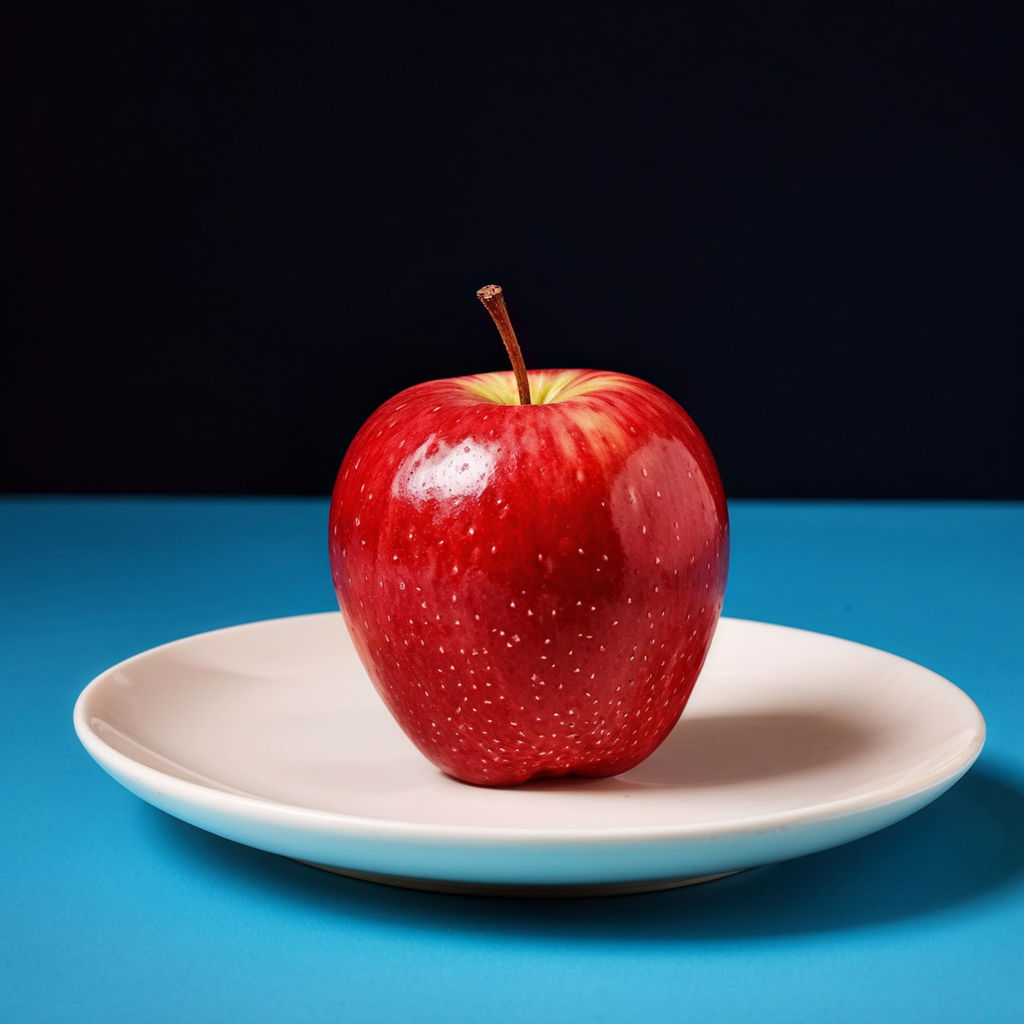
\includegraphics[width=\textwidth]{apple_1.png}
  %Generated by "Playground" AI, playground.com/create
\end{center}

\begin{selectAll}
    \choice[correct]{The apple's weight}
    \choice[correct]{The apple's color}
    \choice[correct]{The apple's volume}
    \choice{The apple's taste}
    \choice[correct]{The length of the apple's stem}
    \choice[correct]{The circumference of the largest horizontal cross-section of the apple}
    \choice{How the apple smells}
\end{selectAll}
\end{exploration}

In order to figure out how we can use vectors to say meaningful things about fruit, like this apple, we first need to get some common terminology and visualization down.

\begin{remark}

  Let's start with some basic terminology. 

\begin{definition}
    \item[Tuples] We can organize the measurements of the apple by encoding values of the apple's useful features as the locations in space. This is what's called a tuple, or more specifically an \textit{ordered tuple}. We more colloquially call these \textit{points} in space, however depending on the context you can equally call them \textit{vectors}.


    \item[An ordered pair] is just a pair of numbers $[a,b]$ delineated by parenthesis (or brackets) with the entries separated by a comma. It's called ``ordered'' because $[a,b] \ne [b,a]$. 
    
    \begin{example}

      In terms of vectors, if $\vec{v}=[3,4]$ and $\vec{w}=[4,3]$, then $\vec{v}\ne \vec{w}$, because the first coordinate of $\vec{v}$ is $3$ and the first coordinate of $\vec{w}$ is $4$.

    \end{example}
    
    \item[An ordered tuple] is just an array (i.e. a list) of an arbitrary, but fixed, number of elements that is ordered like an ordered pair. As before, while some might want to only call these \emph{points} in space, it is often equally useful to just call them \emph{vectors}.
    
    \item[Coordinates:] Each position in the array (e.g first, second, third) is called a \textit{coordinate}. In the vector $[a, b, c]$, we say that $a$ is the first coordinate, $b$ is the second coordinate, and $c$ is the third coordinate. 

\end{definition}
\end{remark}

\begin{remark}

  Next, visualization.

\begin{description}
    \item[How It's Visualized:] 
    
    The apple vectors might be represented by ordered tuples containing measures of the following features: 
    
    $\lbrace \text{weight, color, volume, stem length, max circumference} \rbrace$.
    
    For instance, the vector $\vec{a}$ below is one potential vector representation of an apple

    $$\vec{a}=[\text{weight, color, volume, stem length, max circumference}],$$

    where each entry in the tuple is a number giving the measurement of the apple's feature.

    If we wanted to represent the apple's weight (in grams), stem length (in cm), and circumference (in cm), we might represent the apple as the vector $\vec{a}=[80, 3, 25]$.

    Geometrically, each coordinate gives us one axis in $d$-dimensional space. This is why we call the number of coordinates the \textit{dimension} of the vector. So the vector $\vec{a}=[80, 3, 25]$ would be a 3-dimensional vector, as it lives in 3-dimensional space.

    \begin{definition}\name{The position vector}

      Let $P$ be a tuple location in $n$-dimensional space. The \textbf{position
        vector}%
      \index{position vector} of $P$ is the vector
      $\vec{p}$ whose tail is at the origin and whose tip
      is at $P$.
      \begin{center}
        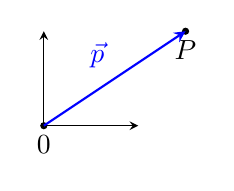
\begin{tikzpicture}[scale=0.6]
          \draw[<->](2,0,0)--(0,0,0)--(0,2,0);
          \draw[fill] (0,0) circle [radius=1.8pt] node[below]{$0$};
          \draw[fill] (3,2) circle [radius=1.8pt] node[below]{$P$};
          \draw[thick, blue, ->](0,0) -- node[above left]{$\vec{p}$} (3,2);
        \end{tikzpicture}
      \end{center}
      If the point $P$ has coordinates $(p_1,\ldots,p_n)$, then the
      components of the position vector are
      \begin{equation*}
        \vec{p} =
        \startmat{c}
          p_1    \\
          \vdots \\
          p_n
        \stopmat.
      \end{equation*}
      Thus, the coordinates of a point are the same as the components of
      its position vector. 
      
      \begin{remark}
      
      For this reason, we will often interchangeably visualize vectors as points in space, or visualize them as arrows. For the purposes of this course, the choice of one over the other is often cosmetic, or a matter of emphasis. If there are too many vectors to nicely visualize at once as arrows, we'll often use points instead.

    \end{remark}
    \end{definition}

    The value in each coordinate tells you how far along its axis you should move.


    %Include a jpg image of a 3-dimensional vector [80, 3, 25] in a 3-dimensional space
    \begin{center}
      %make the width 3/4 of the textwidth
    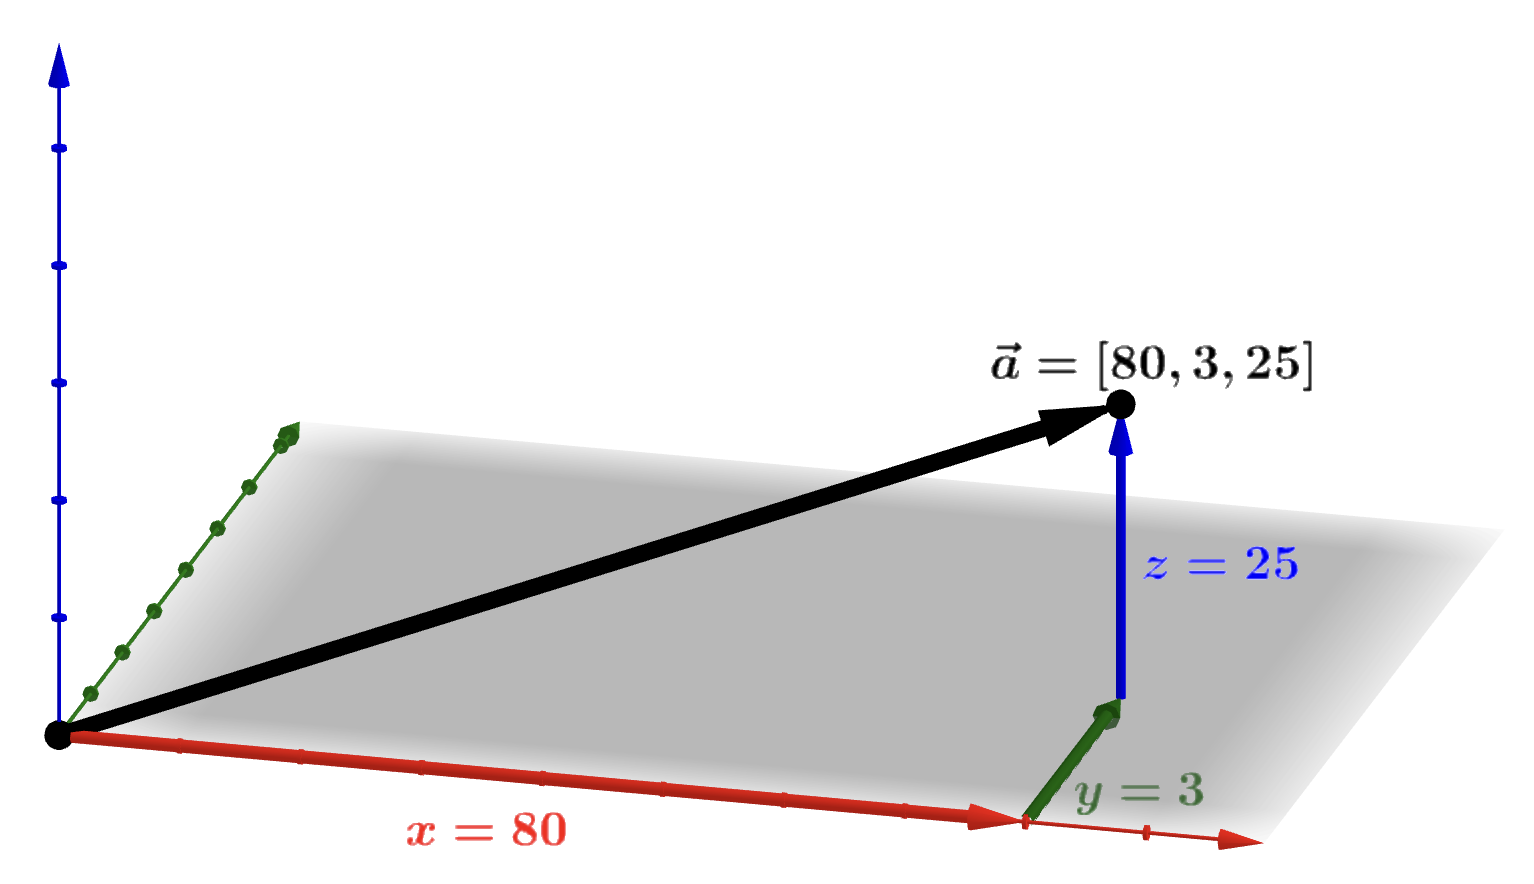
\includegraphics[width=.75\textwidth]{80-3-25_vector.png}
    \end{center}

    You locate our vector $\vec{a}=[80, 3, 25]$ by first moving 80 units along the $x$-axis, then moving 3 units in the direction of the $y$-axis along the $x-y$ plane, and finally moving 25 units in the direction of the $z$-axis in $x-y-z$ space, as seen in Figure BLAH. (Note: the axes are not uniformly scaled in this figure).


\end{description} 
\end{remark}

\begin{exploration}

  Let's say one apple weighs 160 grams (aka 1.6 \emph{decagrams}), has a stem length of 3 cm, and has a circumference of 25 cm (aka 2.5 \emph{meters}). Which of the vectors depicted below could represent the apple? (Select all that apply)

  \choice[correct]{

  \begin{center}
    %make the width 3/4 of the textwidth
    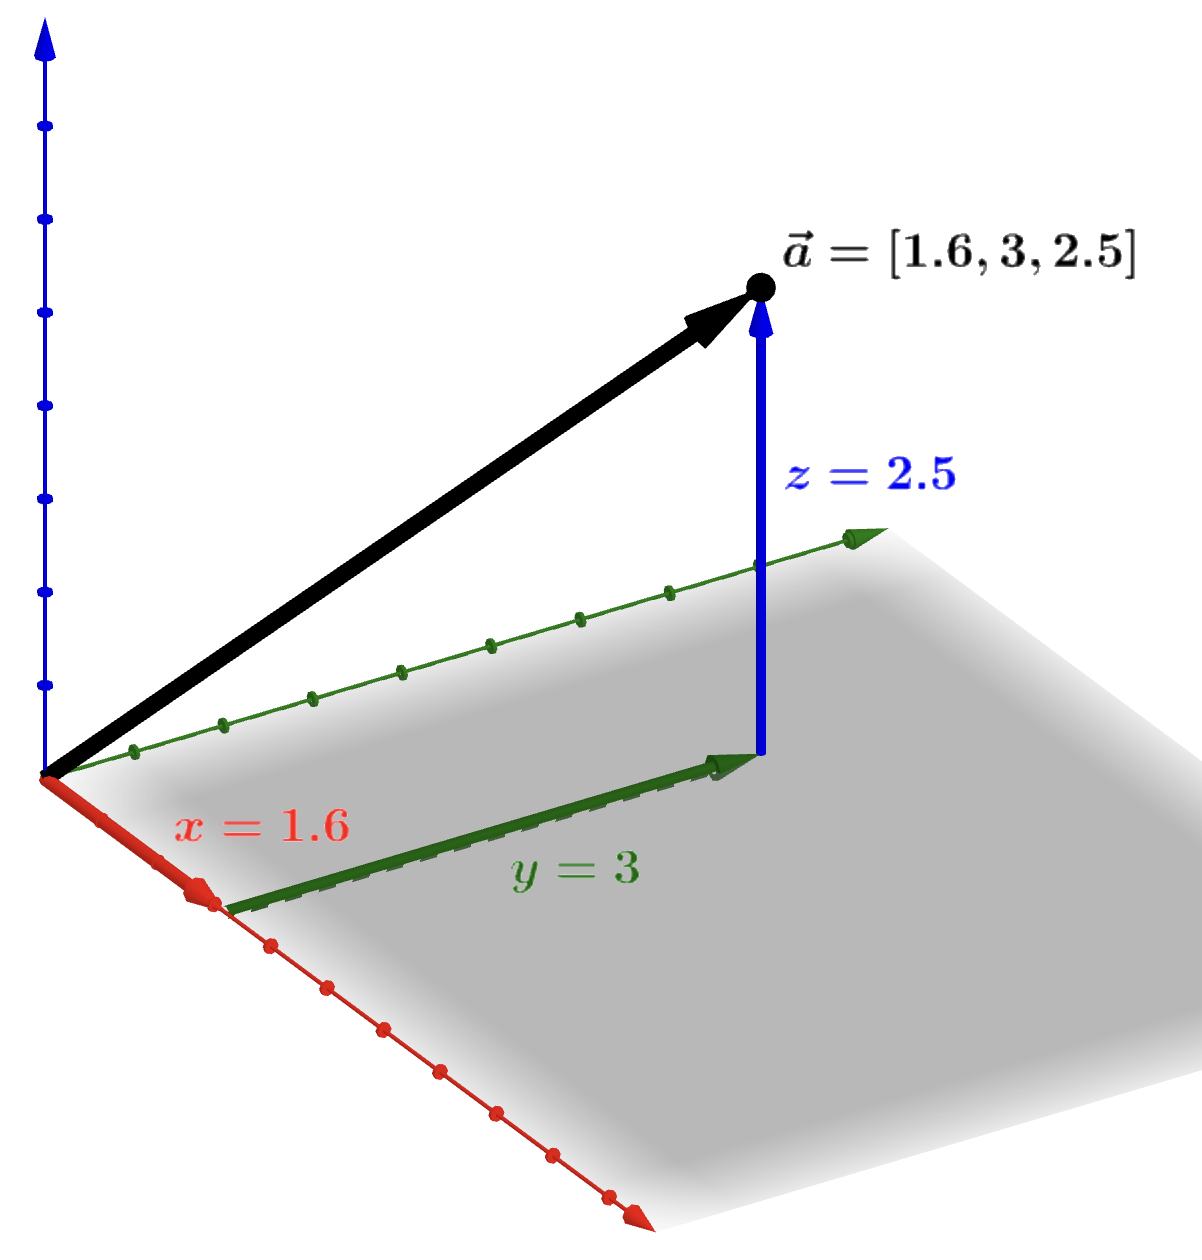
\includegraphics[width=.75\textwidth]{apple_vector_1.png}
  \end{center}
  }
  
\choice[correct]{
    
    \begin{center}
      %make the width 3/4 of the textwidth
    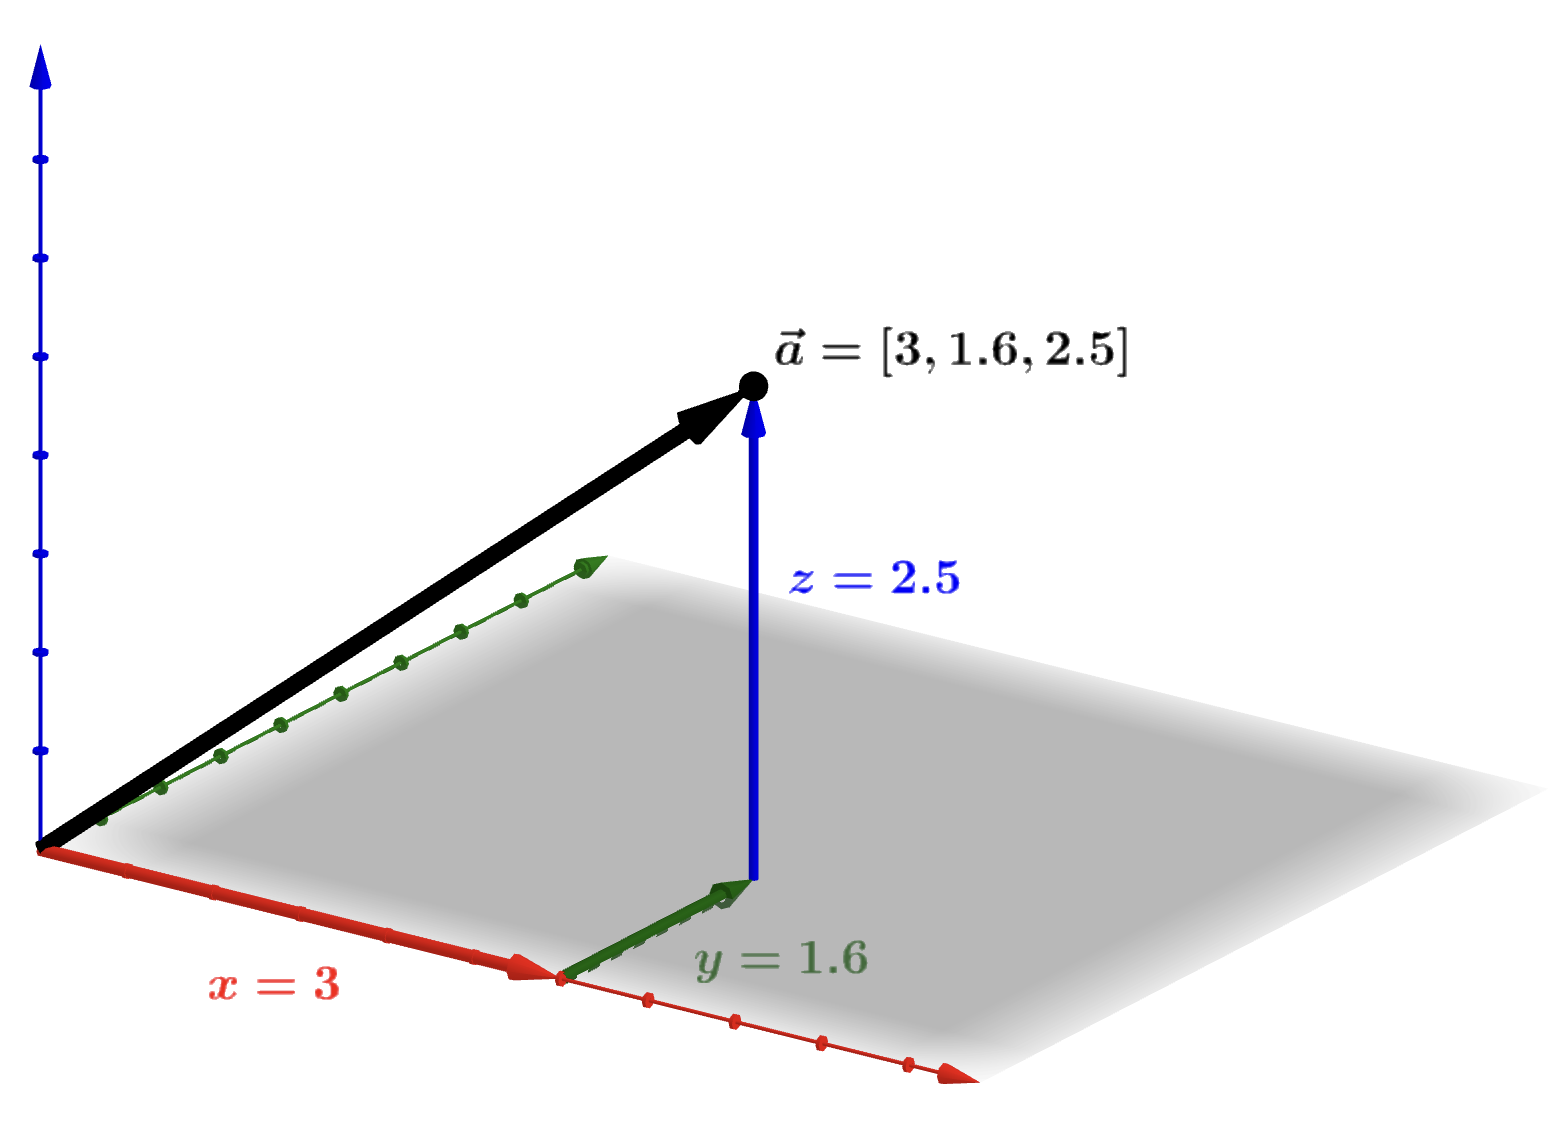
\includegraphics[width=.75\textwidth]{apple_vector_2.png}
    \end{center}
}

\choice[correct]{

  \begin{center}
    %make the width 3/4 of the textwidth
    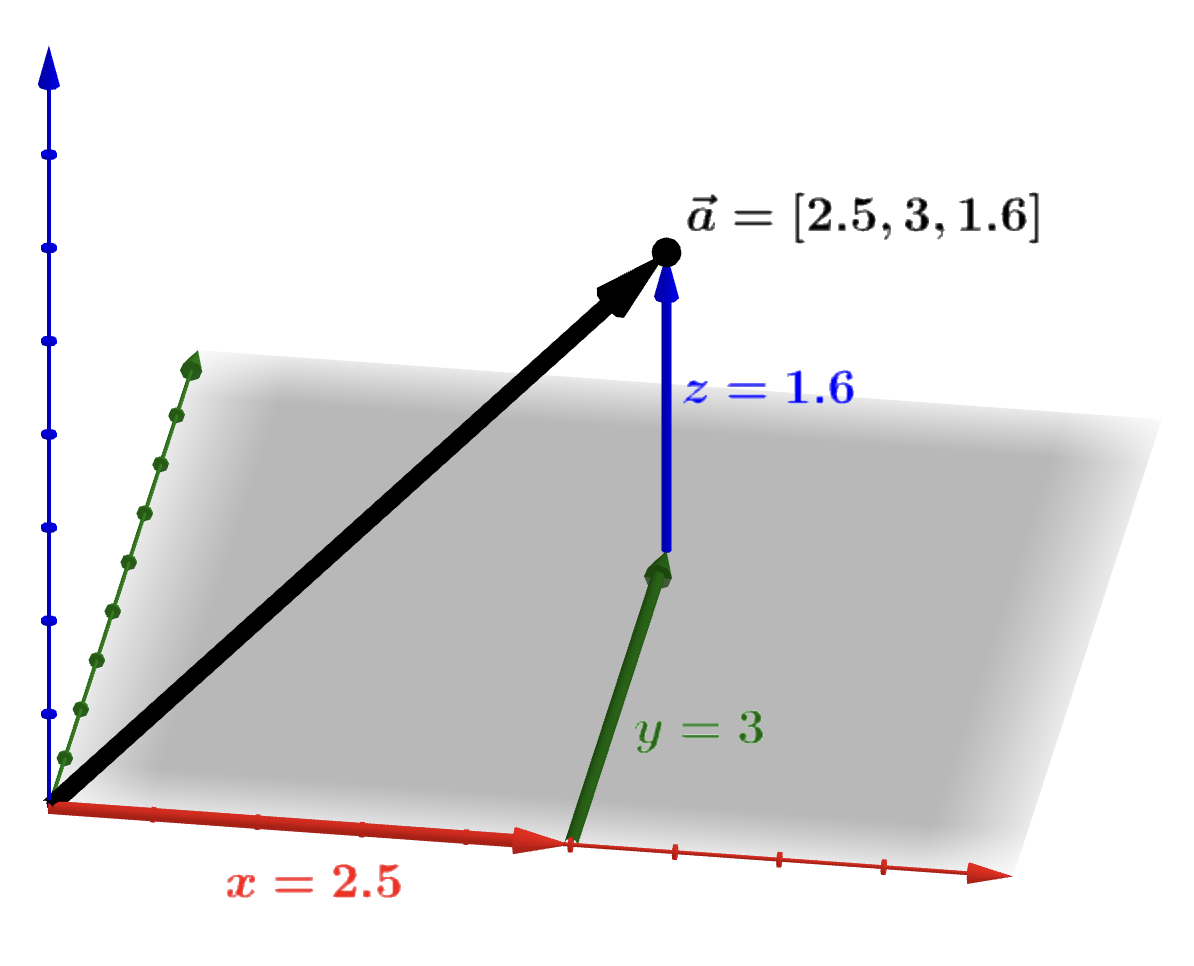
\includegraphics[width=.75\textwidth]{apple_vector_3.png}
  \end{center}

}

\begin{solution}

  All of above could be valid geometric representations of the apple. The main utility is that once each coordinate is assinged a feature (like weight, color, volume, etc.), we want all apples (or fruit for that matter) to have the same ordered features. This way we can compare apples to apples, so to speak, or more generally fruits to fruits.

\end{solution}

\end{exploration}

\begin{exploration}

Finally, let's see one (among countless) application of vector representations.

  A common way to apply vector representations is through classification. This involves making vectors out of the features of objects that you wish to classify (fruits, flowers, houses), and then determining a way to classify multiple objects based on the geometry of the vector representations.


\begin{example}

    Suppose we want to use feature information to compare apples and pears. A data scientist might hope that there's an easy way to geometrically separate all of the apple vectors from pear vectors in a given data set. They'd then use that geometry to predict whether a new fruit is an apple or a pear based on its measurement. 

    It's never as simple geometrically as the GeoGebra environment below, but the idea is the same. We'll do an advanced version of this later in the course when we talk about voting patterns and facial recognition.

    

    \begin{center}
        \pdfOnly{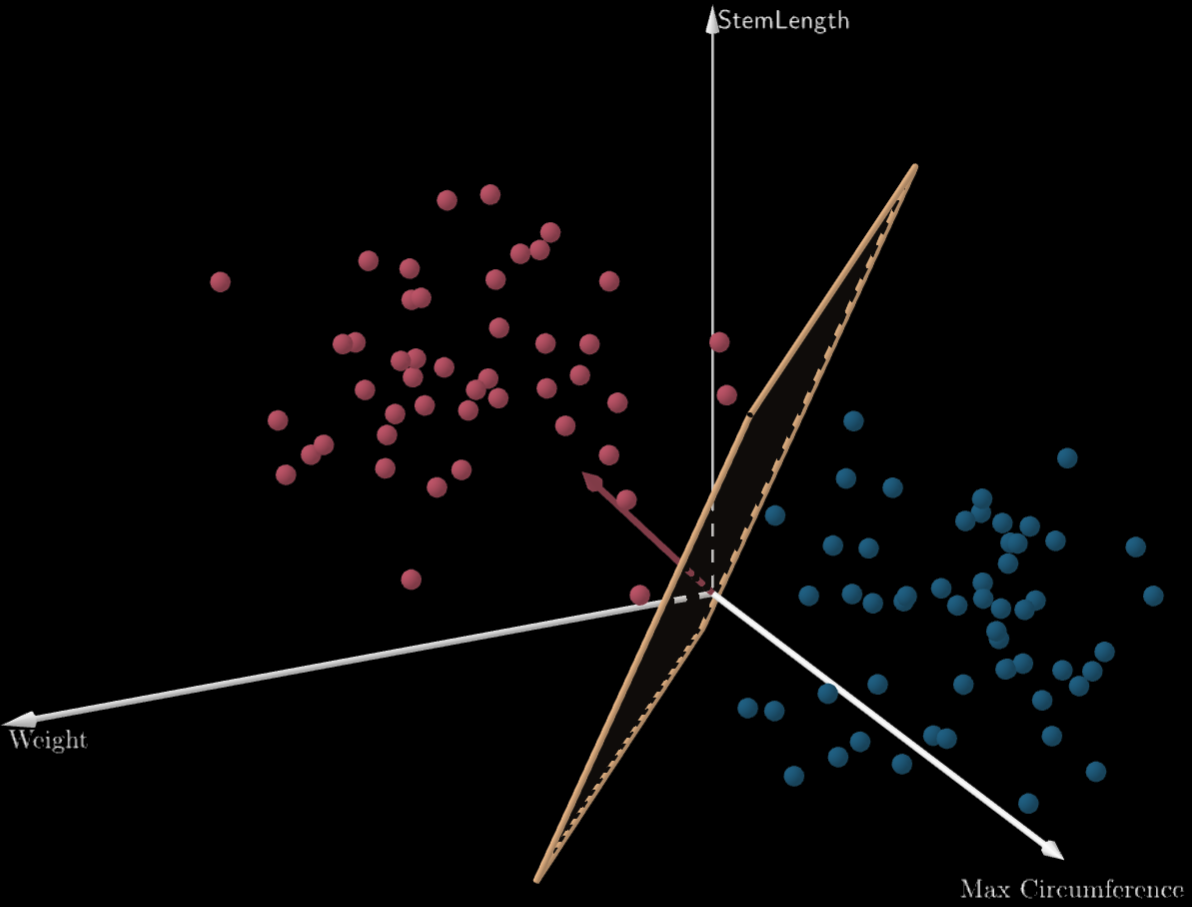
\includegraphics[width=.75\textwidth]{apple-pear.png}\\
        $$\vec{F}\text{ is within the Apple cluster, and is thus an apple rather than a pear.}$$}
        \geogebra{qnghrmdg}{800}{600} %%https://www.geogebra.org/m/qnghrmdg
    \end{center}

    In this very idealistic example, the apple vectors (visualized as red points in 3-D space) cluster together nicely, as do the (blue) pear vectors. You can think of this clustering loosely as the pear vectors generally being closer (distance-wise) to other pears than to apples (we'll talk about this below, and in the homework and discussion).
    
    You can also think of their ``clustering" in terms of a separation in space. If you put a 2-D plane between the apple and pear clusters, the plane cleanly separates the two clusters. We'll revisit this process later in the course as well more explicitly. 
    
    The main point is that the ideas of ``clustering" and ``separation" enable someone to build a program that sorts apples and pears taken from farms en masse based on the feature measurements of the fruit. This exemplifies a powerful use of structure in vectors, that of prediction. As seen in the applet, we don't only care about the apple and pear vectors that we know about, we also care that if we get a new fruit, we can accurately predict whether it's an apple or pear based on the location of its vector representation in 3D space. If it's close to one cluster, or on one side of the plane, and not absurdely far from either cluster (imagine that a banana accidentally got mixed in with the apples and pears), we can predict its type with some confidence.

    
\end{example}
\end{exploration}



\end{document}